\chapter{Получение признаков с использованием нейронных сетей}
\label{chapt2}

Описанный в главе \ref{chapt1} метод получения векторов признаков из столбцов
спектрограммы состоит из нескольких преобразований, каждое из которых опирается
на какие-то свойства музыкальных звукозаписей. Представление спектра звука в
виде вектора признаков необходимо, чтобы облегчить последующую классификацию.
Обучение представлениям -- это раздел машинного обучения, рассматривающий
алгоритмы, направленные на получение наилучших представлений входных данных.
Такие алгоритмы стремятся сохранить наиболее характерные признаки входных данных
в сжатом их представлении.

В основе многих алгоритмов обучения представлениям лежит многослойная нейронная
сеть. Важным свойством таких алгоритмов является возможность предварительного
обучения каждого слоя нейронной сети в отдельности без учителя, на неразмеченных
данных. Благодаря нему требуется существенно меньше размеченных данных для
окончательного обучения нейронной сети в целом.



\section{Теоретические сведения и обзор литературы}

\section{Построение нейронной сети и предобучение при помощи автоассоциаторов}

\section{Построение рекуррентной нейронной сети}

\section{Эксперименты}

%\newpage
%============================================================================================================================
\section{Как вставлять изображения} \label{sect2_2}

\begin{figure} [h] 
  \center
  \includegraphics [scale=0.27] {LaTeX}
  \caption{TeX.} 
  \label{img:latex}  
\end{figure}

А это две картинки под общим номером и названием:
\begin{figure}[h]
  \begin{minipage}[h]{0.49\linewidth}
    \center{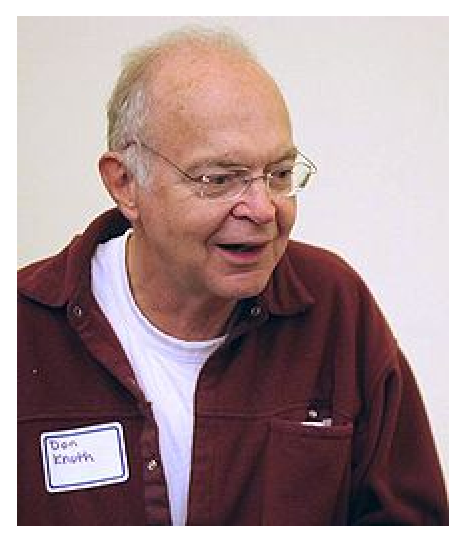
\includegraphics[width=0.5\linewidth]{knuth1} \\ а)}
  \end{minipage}
  \hfill
  \begin{minipage}[h]{0.49\linewidth}
    \center{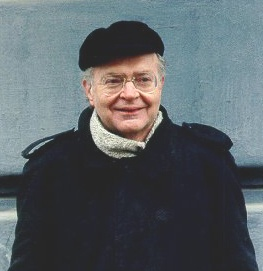
\includegraphics[width=0.5\linewidth]{knuth2} \\ б)}
  \end{minipage}
  \caption{Очень длинная подпись к изображению, на котором представлены две фотографии Дональда Кнута}
  \label{img:knuth}  
\end{figure}

%\newpage
%============================================================================================================================

\clearpage